\chapter{SYSTEM ANALYSIS AND DESIGN}
\section{methodology}
To build a Build Wizard website in Nepal,an agile methodology with an iterative approach would be well-suited.Here's a breakdown of the methodology:
\begin{itemize}
   \item \textbf{Flexibility:}Agile is a flexible approach to project management and development.
   \item \textbf{Customer-Centric:}t prioritizes customer satisfaction and regular customer feedback.
   \item \textbf{Iterative Development:}Projects are divided into small, iterative steps for incremental progress.
   \item \textbf{Collaboration:}Cross-functional teams work closely together, promoting collaboration.
   \item \textbf{Continuous Feedback:}regular feedback loops are essential for improvement.
\end{itemize}

\section{System Analysis}
   \begin{itemize}  
      \item \textbf{Define Requirements and Scope:}
      Gather requirements  considering their needs and preferences.Clearly define the scope of the project, identifying the key features and functionalities.
      \item \textbf{Plan and Design:}
      Create prototypes to visualize the user interface.Plan the overall architecture, database structure, and technology stack for the website.
      \item \textbf{Develop Minimum Viable Product:}
      Start by building the core functionalities required for the Build Wizard, such as component search, filtering, and basic compatibility checks.
      Release an initial version of the website with the essential features to gather user feedback and validate the concept.
      
      \item \textbf{Gather User Feedback:}
      Encourage users to provide feedback on their experience, including usability, features, and any issues they encounter.
      Conduct surveys or user interviews to gain insights into user preferences, and improvements.
      
      \item \textbf{Iterative Development:}
      Based on user feedback, prioritize and implement enhancements and additional features in iterative cycles.
      Continuously refine the user interface, performance, and usability to optimize the website.
      
      \item \textbf{Test and Quality Assurance:}
      Conduct thorough testing to ensure the functionality and compatibility of the website across different devices, browsers, and operating systems.
      Identify and address any bugs, errors, or inconsistencies to improve the website's stability and reliability.
      \item \textbf{Release and Deployment:}
      Deploy the website to a production environment, ensuring proper setup and security measures.Monitor the performance of the website and address any issues that arise after the launch.
      
      \item \textbf{Continuous Improvement:}
      Regularly gather user feedback and track website analytics.
      Plan and implement updates, new features,pricing and component database expansions to keep the website relevant and up to date.
   \end{itemize}
\section{Requirement Analysis}
\subsection{functional Requirements}
\begin{itemize}
   \item \textbf{User Registration:}Users should be able to create accounts and authenticate themselves securely to access personalized features and configurations.
   \item \textbf{PC Component Selection:}Users should be able to browse and select PC components (e.g., CPU, GPU, RAM) from a categorized list.
   \item \textbf{Configuration Building:}Users should be able to add selected components to a configuration list and customize quantities based on their requirements.
   \item \textbf{Real-time Data Updates:}Prices, availability, and specifications of components should be updated in real time from reliable sources.
   \item \textbf{Admin Dashboard:}Admins should have access to a dashboard to manage users, components, reviews, and configurations.
\end{itemize}
\subsection{Non-functional Requirements}
\begin{itemize}
   \item \textbf{Performance:}The system should respond to user interactions within appropriate time to provide a seamless user experience.
   \item \textbf{User Experience and Design:}The user interface should be intuitive, visually appealing, and responsive across various devices and screen sizes.
   The design should follow usability principles, making the platform easy to navigate and understand for users.
\end{itemize}
   \section{Feasibility Analysis}
   The feasibility analysis conducted for the BuildWizard project has shed light on crucial aspects integral to its successful development, deployment, and sustainability. Key findings from each dimension of the analysis are summarized below:
   \begin{itemize}
      \item \textbf{Technical Feasibility:}The technical aspects required for the BuildWizard project, encompassing hardware, software, and technical expertise, are feasible and attainable within the proposed scope.
      \item \textbf{Schedule Feasibility:}A well-structured project timeline has been devised, accounting for necessary phases and potential time constraints to ensure timely completion.
      \item \textbf{Operational Feasibility:}The integration of BuildWizard with existing systems and workflows is feasible, and user acceptance testing will further optimize its operational efficiency.
   \end{itemize}
   \newpage
      \section{ER diagram}
      An Entity-Relationship (ER) diagram is a graphical representation used in database design to illustrate the logical structure and relationships of entities, attributes, and the associations between them within a database system. It serves as a visual tool for modeling and communicating how different components in a database are connected.\\\\
      Figure 3.2 is ER diagram of system it shows the entites of system with their attributes and relationships.
      \begin{figure}[ht]
      \centering
      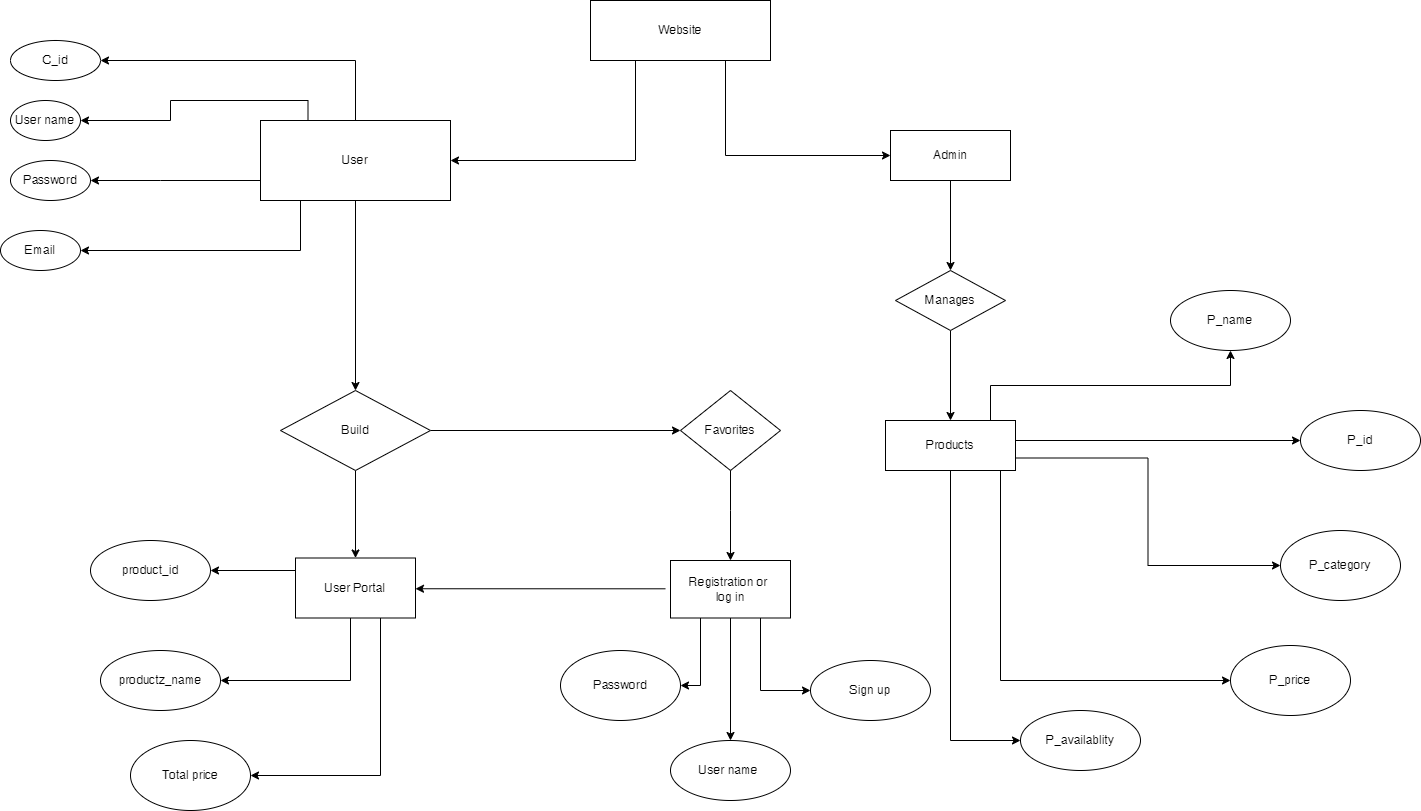
\includegraphics[width=15cm]{Diagrams/Pc_part_er_diagram.drawio.png}
      \caption{ER diagram}
      \end{figure}
      \subsection{Process Modeling(DFD)}
     \begin{figure}[ht]
      \centering
      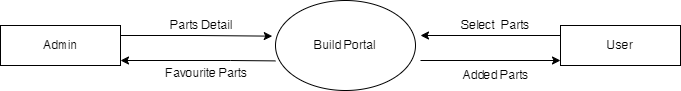
\includegraphics[width=15cm]{Diagrams/0levDFD.drawio.png}
      \caption{DFD diagram}
     \end{figure}
     \newpage
      \section{System Design}
   \subsection{Architecture design}
   Following figure shows the architecture design of this system.It shows what are the functions can be accesses after opening our site.
   \begin{figure}[H]
   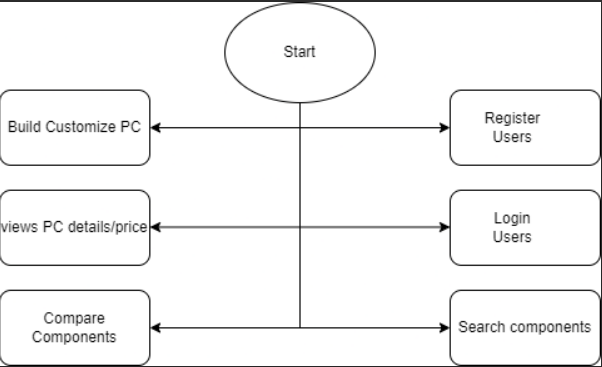
\includegraphics[width=15cm]{Diagrams/arcdesign.png}
   \caption{Architecture design}
   \end{figure}
   \newpage
   \subsection{Database Schema Design}
   Schema design, also known as database design or data modeling, is the process of structuring and organizing the data and relationships within a database system. It involves defining the tables, fields, data types, constraints, and relationships that will be used to store and manage information in a database.\\\\
   \begin{figure}[H]
   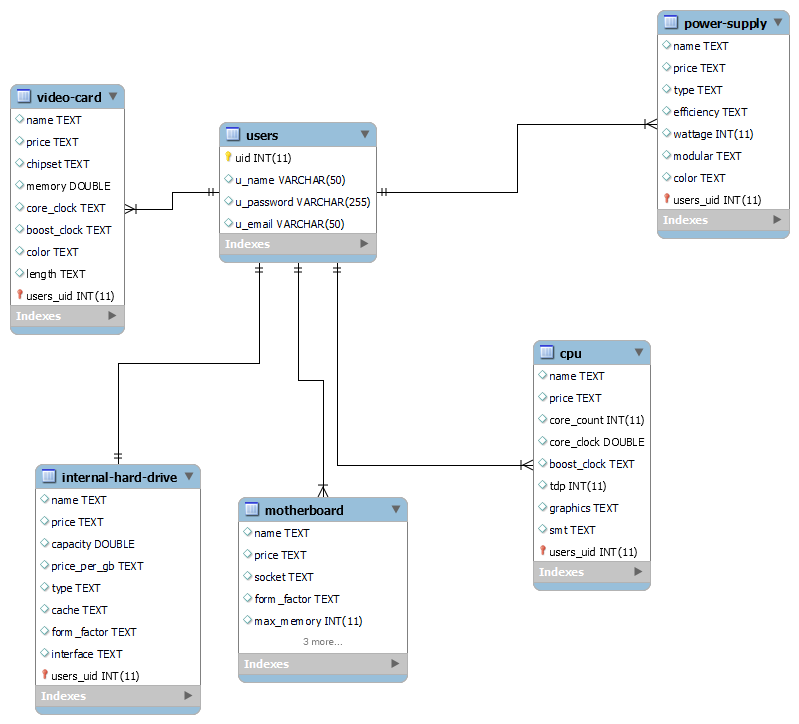
\includegraphics[width=15cm]{Diagrams/schema.png}
   \caption{Database Schema Design}
   \end{figure}
      \subsection{Interface Design}
      User Interface (UI) design is the process of creating the visual layout, appearance, and interactive elements of a digital product, such as a website or application. It focuses on enhancing user experience by crafting a visually pleasing, intuitive, and efficient interface. UI designers select colors, typography, icons, and other visual elements, as well as design the arrangement and behavior of user interface components to ensure a seamless and engaging interaction between users and the product. The goal of UI design is to create an interface that is both aesthetically appealing and user-friendly, facilitating easy navigation and efficient completion of tasks.\\\\
      Given picture shows the Home page of BuildWizard website.\\\\
      \begin{figure}[H]
      \centering
      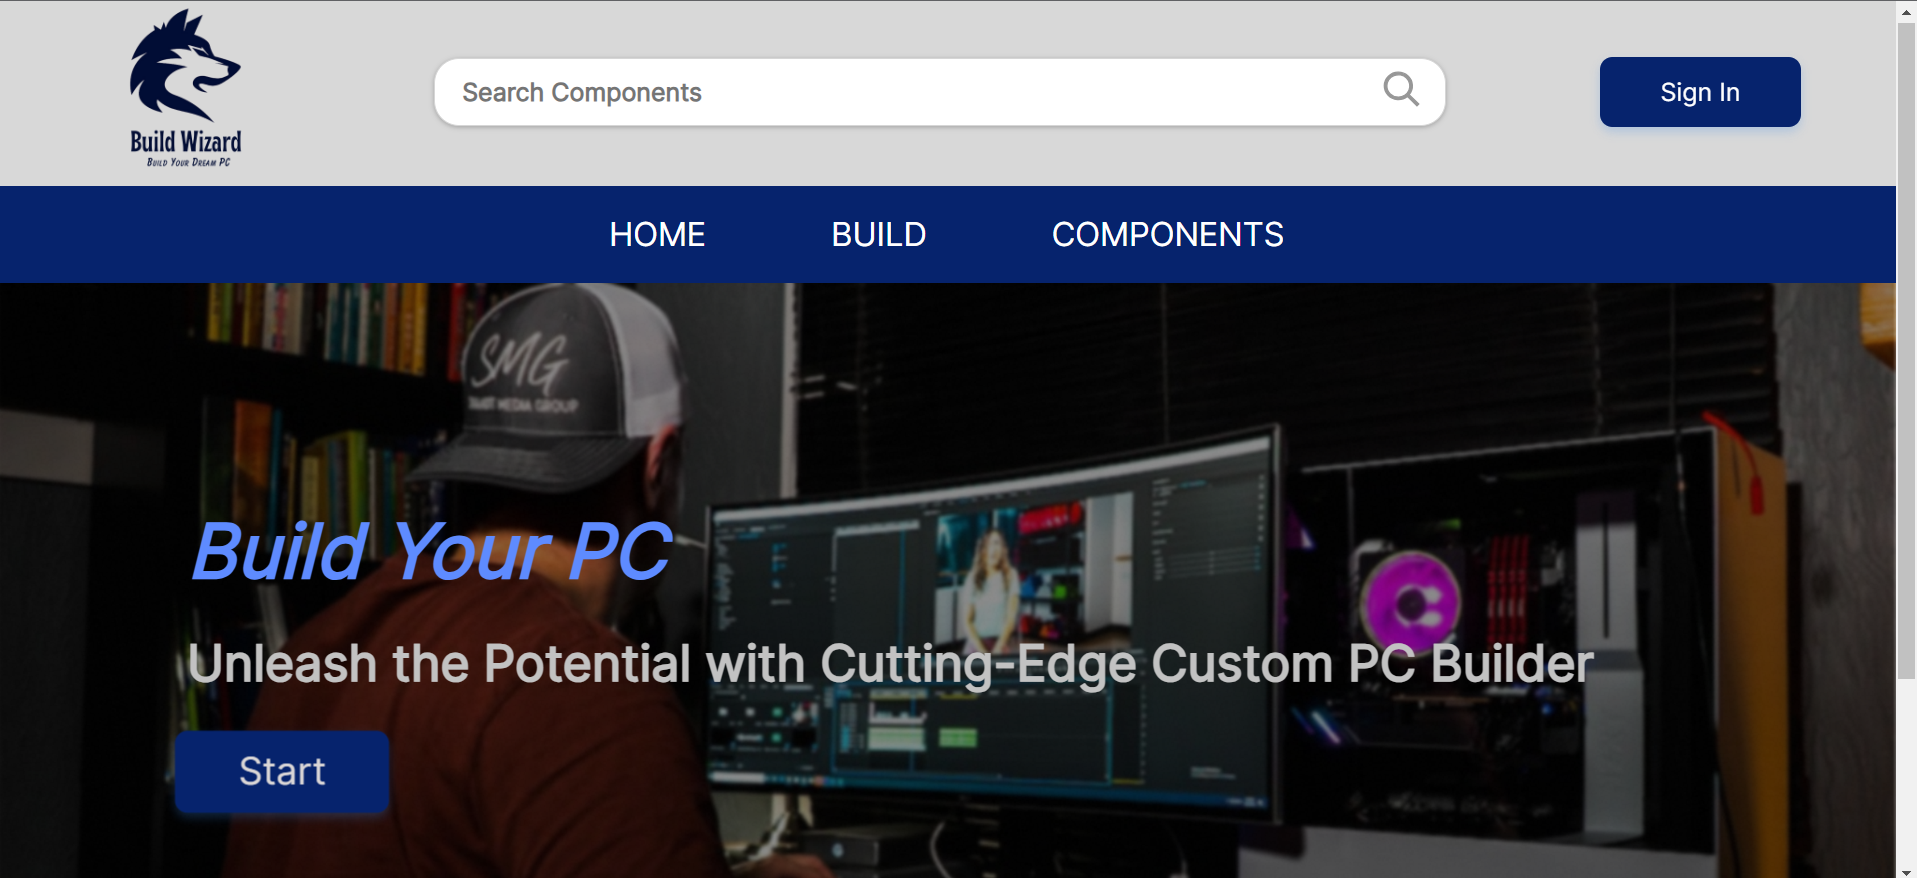
\includegraphics[width=15cm]{Diagrams/UIHOME.png}
      \caption{Interface Design Home page}
      \end{figure}
      
      \newpage
      Below picture shows the UI SignUp page of this website.\\\\
      \begin{figure}[H]
      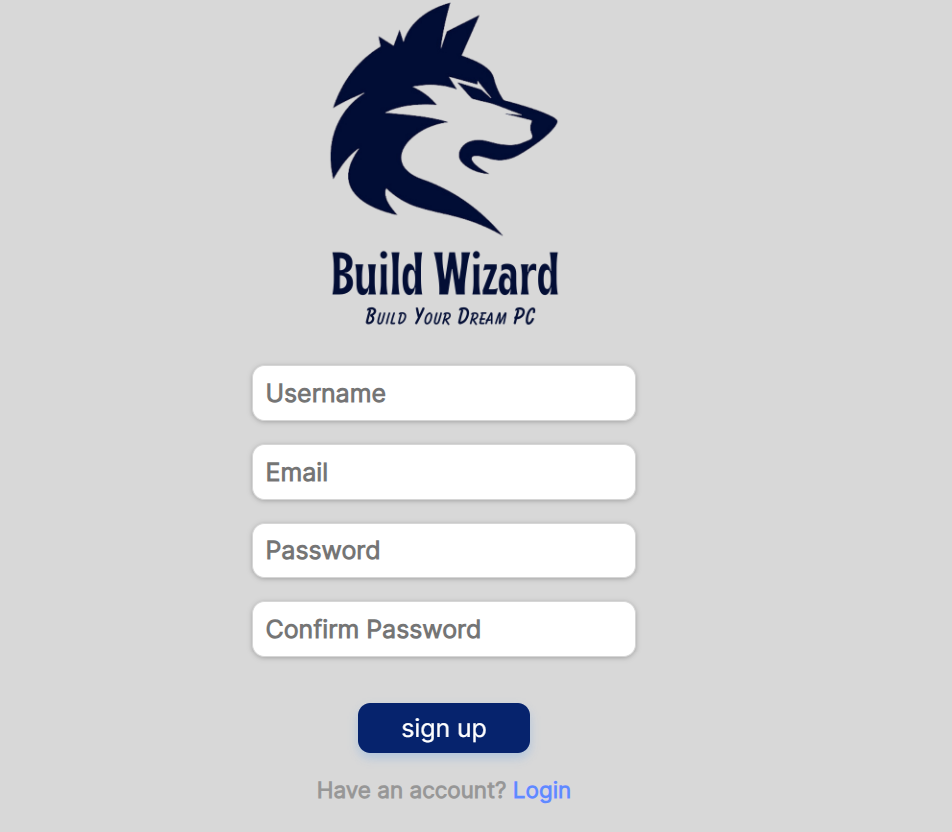
\includegraphics[width=15cm]{Diagrams/UISIGNUP.png}
      \caption{Interface Design SignUp}
      \end{figure}
      \newpage
      Following Picture shows the UI of LogIn on this website.\\\\
      \begin{figure}[H]
      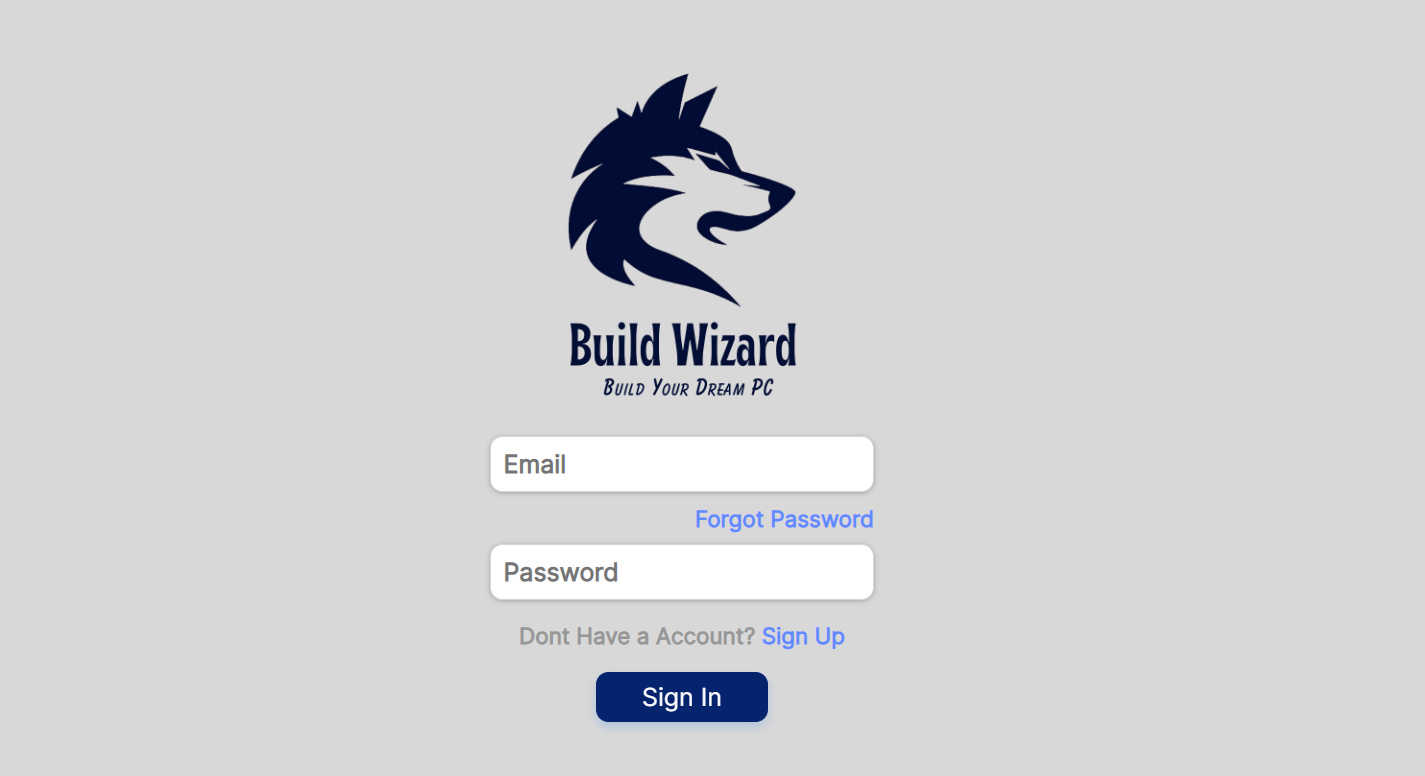
\includegraphics[width=15cm]{Diagrams/UILOGIN.png}
      \caption{Interface Design SignIn}
      \end{figure}
      \subsection{Physical DFD}
      \begin{figure}[H]
         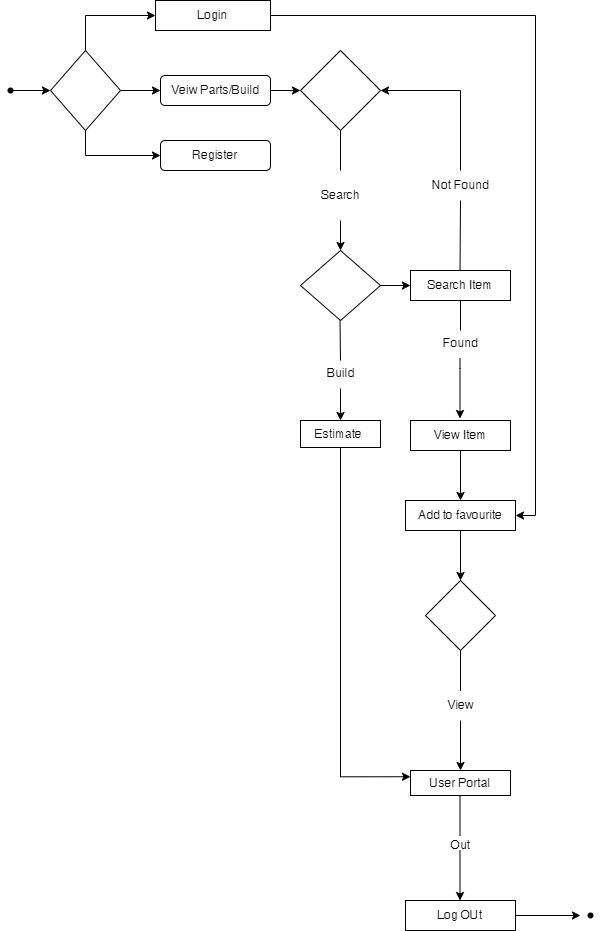
\includegraphics[width=15cm]{Diagrams/physicaldfd.png}
         \caption{Physical DFD diagram}
         \end{figure}
  


      